\chapter{논리적 추론 규칙}

수학 문제를 해결하는 과정을 자세히 살펴보면, 가정으로부터 \textbf{논리적 추론}을 거쳐 결론을 얻는 것을 확인할 수 있다. 그러므로 올바른 문제 해결을 위해서는 \textbf{논리적 추론 규칙과 그 활용 방법}을 이해해야 한다.

명제 \(p \ra q\)가 참일 때, \(p \implies q\) 또는 다음과 같이 표기한다.
\[
    \begin{array}{c|l}
        (1) & p \\\hline & q
    \end{array}
\]
가로선 \(-\)를 기준으로 위에 적힌 것이 가정이고, 아래에 적힌 것이 결론이다. (1)은 가정에 번호를 붙인 것이다. 예를 들어, 가정이 여러 개여서 명제 \(p_1, p_2, p_3 \ra q\)가 참이라면, 다음과 같이 표기한다.
\[
    \begin{array}{c|l}
        (1) & p_1 \\ (2) & p_2 \\ (3) & p_3 \\\hline & q
    \end{array}
\]

또한 가정에 포함된 내용은 참으로 받아들이고 시작한다.

\pagebreak

\section{명제 사용하기}

가장 기본적인 추론 규칙이다.
\[
    \begin{array}{c|l}
        (1) & p \ra q \\ (2) & p \\\hline & q
    \end{array}
\]
\(p \ra q\)가 참임을 아는 상황에서, \(p\)가 참이라면, 당연히 \(q\)가 참일 것이다.

간단한 추론 규칙이기 때문에, 이 규칙만을 사용하는 문제는 개념 확인 문제에서나 만나겠지만, 추론 규칙들의 가장 기본이 되기 때문에 중요하다. 이 규칙을 사용하기 위해서는 문제의 가정 \(p\)와 결론 \(q\)를 파악하고 \(p \ra q\) 형태의 명제를 배운 적이 있는지 찾아야 한다. 해당 형태의 명제를 찾으면, 그 명제를 사용하여 바로 답을 얻고 문제를 해결할 수 있다. 다음 예제를 살펴보자.

\bigskip

\ex. 가로의 길이가 5이고 세로의 길이가 7인 직사각형의 넓이를 구하여라.

\sol 위 문제에서 가정 \(p\)와 결론 \(q\)를 찾아 명제 \(p \ra q\)의 형태로 바꾸면 다음과 같다.
\begin{center}
    \(\underset{p}{\underline{\text{가로의 길이가 5이고 세로의 길이가 7인 직사각형}}}\text{에 대하여 } \underset{q}{\underline{\text{직사각형의 넓이는 [...]이다.}}}\)
\end{center}
배운 명제 중 위와 같은 형태를 가진 명제를 찾아보면 다음과 같다.
\begin{center}
    \(\underset{\text{가정}}{\underline{\text{가로의 길이가 } a\text{이고 세로의 길이가 }b\text{인 직사각형}}}\text{에 대하여 } \underset{\text{결론}}{\underline{\text{직사각형의 넓이는 } ab\text{이다.}}}\)
\end{center}
여기서 \(a = 5\), \(b = 7\)로 두면 다음과 같다.
\begin{center}
    \(\underset{p}{\underline{\text{가로의 길이가 5이고 세로의 길이가 7인 직사각형}}}\text{에 대하여 } \underset{q}{\underline{\text{직사각형의 넓이는 35이다.}}}\)
\end{center}
위 명제 \(p \ra q\)는 참이고, 문제의 가정에 의해 \(p\)가 참이므로 [명제 사용하기] 규칙에 의해 \(q\)가 참이다. 따라서 직사각형의 넓이는 \(35\)이다. \qed

\bigskip

너무 쉬운 문제를 복잡하게 풀었다는 생각이 들 수도 있겠지만, 문제 자체보다는 과정과 추론 규칙을 사용하는 사고의 흐름에 주목하자. 위 풀이 과정은 크게 3단계로 나눌 수 있다.

\begin{enumerate}
    \item 주어진 것과 구하는 것을 파악한다.
    \item \textbf{주어진 것과 구하는 것을 바탕으로} 배운 명제 중 적용할 수 있는 것이 있는지 찾아본다.
    \item \textbf{논리적 추론 규칙을 사용한다.}
\end{enumerate}

이와 같은 과정은 위 예제 뿐만 아니라 \textbf{모든 수학 문제에 적용 가능한 방법}이다. 단, 문제가 복잡해지면 (2), (3)단계를 반복적으로 적용한다는 점이 달라진다.

\pagebreak

많은 학생들이 어려워하는 단계는 (2)단계이다. 배운 내용 중 어떤 내용을 적용해야 할지 어떻게 잘 찾을 수 있을까? 혹시 문제 속에 답이 있다는 농담 같은 진담을 들어본 적이 있는가? 핵심은
\begin{center}
    \textbf{주어진 것과 구하는 것을 바탕으로}
\end{center}
적용할 명제를 찾아야 한다는 점이다. \textbf{문제에서 주어진 조건들이 곧 힌트가 된다.}

위 예제의 경우에 이를 적용해 보자. 문제의 가정에는 직사각형의 가로와 세로 길이가 주어져 있다. 그리고 결론으로 구하는 것은 직사각형의 넓이이다. 따라서 배운 것 중에서 `직사각형의 가로/세로 길이', `직사각형의 넓이'와 관련된 내용을 찾아보면 된다. 그러면 다음과 같은 질문을 할 수 있을 것이다.
\begin{itemize}
    \item (주어진 것 바탕으로) 직사각형의 가로/세로 길이를 가지고 무엇을 할 수 있을까?
    \item (구하는 것 바탕으로) 직사각형의 넓이를 구하는 방법으로 무엇을 배웠었나?
\end{itemize}
위와 같은 질문을 하며 생각하다 보면 결국 위 풀이 과정에서 사용한 넓이 공식(명제)이 자연스럽게 떠오르게 될 것이다. 실제로 두 번째 질문에 대한 답을 생각해 보면, 직사각형의 넓이를 구하는 여러 방법 중 몇 가지가 떠오른다.
\begin{enumerate}
    \item 가로의 길이가 \(a\), 세로의 길이가 \(b\)이면 넓이는 \(ab\)이다.
    \item 대각선의 길이가 \(x\)이고 두 대각선이 이루는 예각이 \(\theta\)이면 넓이는 \(\frac{1}{2}x^2 \sin \theta\)이다.\footnote{사각형의 두 대각선의 길이가 \(a, b\)이고 대각선이 이루는 예각의 크기가 \(\theta\)일 때, 사각형의 넓이는 \(\frac{1}{2}ab\sin\theta\)이다.}
\end{enumerate}
어느 것을 써야 할까? 당연히 (1)번이고, 그 이유는 \textbf{주어진 것을 바탕으로 생각}해야 하기 때문이다.  이처럼 \textbf{주어진 것과 구하는 것을 바탕으로} 생각해야 빠르고 효율적으로 적용할 명제를 찾을 수 있다.

% 일반적으로 (1)번은 어렵지 않지만, (2)번과 (3)번은 결코 단순한 작업이 아니다. 학년이 올라가며 배우는게 많아지고 복잡해질수록 적용할 명제를 찾는 과정은 더 어려워지기 때문에 문제에 대한 접근 방법이 떠오르지 않을 수도 이다. 또한, 논리적 추론 규칙을 올바르게 적용했다고 하더라도 문제가 원하는 결론에 도달하지 못해 풀다가 막힐 수도 있다.

\medskip

다음 예제에서 가정 \(p\)와 결론 \(q\)를 찾고, 사용한 명제 \(p \ra q\)를 서술하여라.

\ex. 오각형의 대각선의 개수를 구하여라.

\vspace*{80px}

\ex. 반지름의 길이가 \(3\)인 원의 넓이를 구하여라.

\vspace*{80px}

\pagebreak

\section{삼단논법}

수학 전반에서 가장 많이 사용되는 추론 규칙이다.
\[
    \begin{array}{c|l}
        (1) & p \ra q \\ (2) & q \ra r \\ (3) & p \\\hline & r
    \end{array}
\]

당연한 것 같지만, 왜 그런지 살펴보자.

\pf \(p \ra q\), \(q \ra r\)이 모두 참임을 아는 상황에서, \(p\)가 참이라고 하자. 그러면 [명제 사용하기]를 가정 (1), (3)에 적용하면 \(q\)가 참임을 알 수 있다. 그러면 현재 상태는 다음과 같다.
\[
    \begin{array}{c|l}
        (1) & p \ra q \\ (2) & q \ra r \\ (3) & p \\ (4) & q \\\hline & r
    \end{array}
\]
[명제 사용하기]를 가정 (2), (4)에 적용하여 \(r\)이 참임을 알 수 있다. \qed

이 추론 규칙을 사용하는 문제에서는 가정 \(p\)와 결론인 \(r\)만 주어지는 경우가 많다. \textbf{그러므로 결론인 \(r\)을 얻기 위해 학생들은 \(p\)와 \(r\)의 징검다리 역할을 하는 \(q\)를 찾아야 한다.} 단, \(p \ra q\), \(q \ra r\)이 모두 참인 \(q\)를 찾아야 한다.

이와 같은 \(q\)를 찾기 위해서는 다음 두 가지를 생각하면 좋다.
\begin{enumerate}
    \item 배운 내용 중 가정이 \(p\)인 명제가 있었나?
    \item 배운 내용 중 결론이 \(r\)인 명제가 있었나?
\end{enumerate}

어려운 문제에서는 가정과 결론의 징검다리 역할을 하는 \(q\)를 여러 개 찾아야 하는 경우도 있다. 이 경우에도 결국에는 문제에 주어진 가정과 결론을 고려하여 그와 관련된 \(q\)를 선택하면 된다.

\pagebreak

다음 예제에서 가정 \(p\)와 결론 \(r\)을 찾고, 징검다리 \(q\)와 사용한 명제 \(p \ra q\), \(q \ra r\)을 서술하여라. 필요하다면 징검다리를 여러 번 사용해도 좋다!

\ex. 방정식 \(3x + 2 = 8\)을 풀어라.

\vspace*{200px}

\ex. 다음 직각삼각형에서 \(\angle x\)의 크기를 구하여라.

\begin{flushright}
    \usetikzlibrary{positioning}
    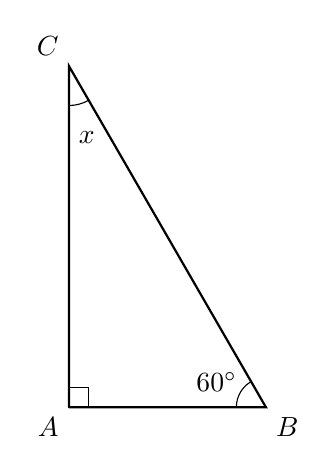
\begin{tikzpicture}[scale=2.5]
        \coordinate (A) at (0, 0);
        \coordinate (B) at (1, 0);
        \coordinate (C) at (0, 1.732);
        \draw[thick] (A) -- (B) node[below right] {\(B\)}
             -- (C) node[above left] {\(C\)}
             -- (A) node[below left] {\(A\)};
        \draw (A) rectangle (0.1, 0.1);
        \draw ([shift=(120:0.15)] B) arc (120:180:0.15);
        \draw ([shift=(270:0.2)] C) arc (270:300:0.2);
        \node at (0.75, 0.13) {\(60^\circ\)};
        \node at (0.09, 1.37) {\(x\)};
    \end{tikzpicture}
\end{flushright}

\pagebreak

\section{대우 사용하기}

명제와 그 대우는 참/거짓을 같이 한다. 명제가 참이면 대우도 참이고, 명제가 거짓이면 대우도 거짓이다. 이를 다음과 같이 표현할 수 있다.
\[
    (p \ra q) \implies (\sim q \ra \sim p)
\]
삼단논법을 사용하여 다음이 성립함을 보여라.
\[
    \begin{array}{c|l}
        (1) & p \ra q \\ (2) & \sim q \\\hline & \sim p
    \end{array}
\]

\ex. 자연수 \(n\)에 대하여 \(n^2\)이 홀수이면 \(n\)이 홀수임을 보여라.

\quad \textbf{대우}:

\pagebreak

\section{그리고}

\textbf{\(p\)와 \(q\)가 모두 참인 경우에만} `\(p\) 그리고 \(q\)'가 참이다. 기호로는 \(p \wedge q\)로 나타낸다.
\[
    \begin{array}{c|l}
        (1) & p  \\ (2) & q \\\hline & p \wedge q
    \end{array}
\]
`\(p\) 그리고 \(q\)'를 증명해야 하는 경우, \textbf{\(p\)와 \(q\)가 모두 성립함을 보이면 된다.}

또한 `그리고'의 정의로부터 다음이 성립한다.
\[
    \begin{array}{c|l}
        (1) & p \wedge q \\\hline & p
    \end{array}
    \qquad
    \begin{array}{c|l}
        (1) & p \wedge q \\\hline & q
    \end{array}
\]
문제에서 조건이 여러 개 주어진 경우 그 중 하나만 택하여 사용할 수도 있다는 의미이다.

\bigskip

다음 예제에서 \(p \wedge q\) 형태의 조건을 사용해 명제로 나타내고, 풀이에 사용한 명제를 서술하여라.

\ex. 2의 배수이고 3의 배수이면 6의 배수임을 보여라.

\vspace*{180px}

\ex. 연립방정식 \(\ds \begin{cases}
    x + y = 4 \\ x - y = 2
\end{cases}\) 를 풀어라.

\pagebreak

\section{또는}

\textbf{\(p\)와 \(q\) 중 적어도 하나가 참인 경우에만} `\(p\) 또는 \(q\)'가 참이다. 기호로는 \(p \vee q\)로 나타낸다. 정의로부터 \(p\)와 \(q\) 중 하나가 참이면 `\(p\) 또는 \(q\)'는 자동으로 참이므로 다음이 성립한다.
\[
    \begin{array}{c|l}
        (1) & p \\\hline & p \vee q
    \end{array}
    \qquad
    \begin{array}{c|l}
        (1) & q \\\hline & p \vee q
    \end{array}
\]

\subsection{경우 나누기 규칙}

다음 규칙은 주로 \textbf{경우를 나눌 때} 사용한다. `\(p_1\) 또는 \(p_2\)'가 참임을 안다고 하자. \(p_1\)이 참일 때 \(q\)가 참이고, \(p_2\)가 참일 때도 \(q\)가 참이라면, \(q\)는 참일 것이다.
\[
    \begin{array}{c|l}
        (1) & p_1 \vee p_2 \\ (2) & p_1 \ra q \\ (3) & p_2 \ra q \\\hline & q
    \end{array}
\]
\textbf{\(p_1\), \(p_2\)가 각각 참인 경우로 나누었을 때, 모든 경우에 대해 \(q\)가 성립하기 때문이다.}

단, \textbf{경우를 빠짐없이 나누었는지 확인해야 한다.} 예를 들어, \(x\)가 실수인 경우 `\(x > 0\) 또는 \(x < 0\)'으로 경우를 나누게 되면 \(x = 0\)인 경우를 빠뜨리게 되므로 주의해야 한다. 만약 경우를 2개 이상으로 나눈다면 각 경우마다 \(q\)가 참임을 보이면 될 것이다.

문제는 주로 \(p \ra q\) 형태로 주어지기 때문에 \(p = p_1 \vee p_2\)이면서 \(p_1 \ra q\), \(p_2 \ra q\)가 참인 \(p_1\), \(p_2\)를 찾아야 할 것이다. 다음 예제에서 조건 \(p\), \(p_1\), \(p_2\), \(q\)를 찾아보라.

\bigskip

\ex. 자연수 \(n\)에 대하여 \(n(n + 1)\)은 짝수이다.

\pagebreak

위 규칙을 강화한 다음 규칙도 종종 사용된다. 앞 규칙과 비교하면, (2)번과 (3)번 조건의 결론 부분이 다르고 결론도 달라진 것을 확인할 수 있다.
\[
    \begin{array}{c|l}
        (1) & p_1 \vee p_2 \\ (2) & p_1 \ra q_1 \\ (3) & p_2 \ra q_2 \\\hline & q_1 \vee q_2
    \end{array}
\]
`\(p_1\) 또는 \(p_2\)'가 참이라고 하자. 여기서 \(p_1 \ra q_1\), \(p_2 \ra q_2\)가 참이라면, \textbf{\(p_1\), \(p_2\) 중 적어도 하나는 참이므로 \(q_1\)과 \(q_2\) 중 적어도 하나가 참}이다. 따라서 \(q_1 \vee q_2\)가 참이어야 한다.

위와 같은 형태의 경우 나누기는 주로 \textbf{각 경우에 대해 다른 전략을 사용하고 그 결과를 합쳐야 하는 경우} 사용된다. 다음 예제에서 조건 \(p\), \(p_1\), \(p_2\), \(q_1\), \(q_2\)를 찾아보라.

\bigskip

\ex. \(x\)에 대한 방정식 \(ax + b = 0\)을 풀어라.

\pagebreak

\subsection{경우 제거하기 규칙}

`또는'과 관련된 마지막 규칙은 \textbf{경우 제거하기 규칙}이다. `\(p\) 또는 \(q\)'가 참일 때, \(p\)가 아니라면 \(q\)가 참이어야 할 것이다. 물론 그 반대의 경우도 당연히 성립한다.
\[
    \begin{array}{c|l}
        (1) & p \vee q \\ (2) & \sim p \\\hline & q
    \end{array}
    \qquad
    \begin{array}{c|l}
        (1) & p \vee q \\ (2) & \sim q \\\hline & p
    \end{array}
\]
예를 들어, 풀이 과정에서 `\(p\) 또는 \(q\)'가 참임을 알았을 때, \(p\)가 논리적으로 모순이거나 문제의 조건에서 \(p\)를 제외하라고 했다면 \(q\)만 고려하면 된다는 의미이다. 다음 예제에 적용해 보라.

\bigskip

\ex. 좌표평면 위의 두 점 \(\rm{A}(1, -1)\), \(\rm{B}(1, 1)\)에 대하여 일차함수 \(y = ax\)가 선분 \(\overline{\rm{AB}}\)와 만나도록 하는 양수 \(a\)의 범위를 구하여라.

\pagebreak

\section{필요충분조건}

\textbf{\(p \implies q\) 그리고 \(q \implies p\)인 경우}, 간단히 \(p \iff q\)로 표기하며 \(p\)는 \(q\)이기 위한 필요충분조건이라 한다. 예를 들어, 다음과 같은 명제가 필요충분조건 형태의 명제이다.
\begin{center}
    실수 \(a, b\)에 대하여, \(ab = 0 \iff a = 0\) 또는 \(b = 0\).
\end{center}

\(p \iff q\)의 정의로부터
\begin{center}
    \(p \implies q\) 그리고 \(q \implies p\)
\end{center}
이다. 즉, 필요충분조건인 명제는 양방향으로 사용이 가능하다!

실제로 문제를 푸는 과정에서는 \(p\)가 가정으로 주어졌을 때, \(p \iff q\)인 명제를 알고 있다면 \(q\)도 가정에 추가하여 사용할 수 있게 된다.

\bigskip

\ex. 이차방정식 \(x^2 + 3x + 2 = 0\)을 풀어라.

\pagebreak

\section{모든}

\textbf{주어진 성질 \(p(x)\)가 모든 \(x\)에 대해 성립할 때}, 다음과 같이 표현한다.
\begin{center}
    \textbf{모든} \(x\)에 대하여 \(p(x)\)이다.
\end{center}
앞 부분과 달리 \(p\)에 변수 \(x\)가 들어간 것은 조건이 \(x\)를 변수로 포함하고 있기 때문이다. 예를 들어,
\begin{center}
    모든 자연수 \(n\)에 대하여 \(n > 0\)이다.
\end{center}
와 같은 명제를 생각할 수 있을 것이다.

`모든'을 포함한 명제는 말 그대로 모든 경우에 성립하므로 굉장히 강력한 명제이다. 강력한 명제는 다양한 곳에서 사용되기 때문에 반드시 기억해야 한다. 단, 여기서 \textbf{`모든'의 범위가 어디인지 주의}해야 한다. 명제 `모든 \textbf{정수} \(n\)에 대하여 \(n > 0\)이다'는 거짓이다!

`모든'을 포함한 명제를 활용하는 방법은 간단하다. \textbf{명제가 제한한 범위에 해당하는 \(x\)를 가져오면 \(p(x)\)가 참임을 사용할 수 있게 된다!} 다음과 같이 변수가 2개인 경우도 살펴보자.
\begin{center}
    (모든) 음이 아닌 실수 \(x, y\)에 대하여, \(\sqrt{xy} = \sqrt{x}\sqrt{y}\)이다.
\end{center}
\(\sqrt{3}\sqrt{5} = \sqrt{15}\)와 같은 계산을 할 때 `모든' 형태의 명제를 사용하고 있었던 것이다. 위에서 \(x = 3\), \(y = 5\)로 둔 경우이다. 변수가 3개인 경우도 마찬가지이다. 다음 예제를 통해 직접 확인해 보라.

사용한 `모든' 형태의 명제를 서술하고, 명제의 각 변수를 어떤 값으로 두었는지 명시하여라.

\bigskip

\ex. \(3^2 \times 3^4 = 3^6\)인 이유를 설명하여라.

\pagebreak

\section{어떤}

\textbf{주어진 성질 \(p(x)\)를 만족하는 \(x\)가 존재할 때}, 다음과 같이 표현한다.
\begin{center}
    \textbf{어떤} \(x\)에 대하여 \(p(x)\)이다.
\end{center}
예를 들어, 다음과 같은 명제가 `어떤'을 포함한 명제이다.
\begin{center}
    어떤 정수 \(x\)에 대하여 \(x^2 - 4x - 5 = 0\)이다.
\end{center}
`모든'과 `어떤'을 모두 사용한 형태도 가능하다.
\begin{center}
    모든 짝수 \(n\)에 대하여, 어떤 자연수 \(k\)에 대하여 \(n = 2k\)이다.
\end{center}

`어떤'을 포함한 명제는 조건 \(p(x)\)를 만족하는 \(x\)가 적어도 하나 존재함을 말해준다. 즉, \textbf{존재성}과 관련된 조건이 곧 `어떤' 형태의 명제이다. `모든'을 포함한 명제의 경우와 마찬가지로, \textbf{조건을 만족하는 \(x\)가 어떤 범위의 \(x\)인지 주의}해야 한다. 명제 `어떤 \textbf{실수} \(x\)에 대하여 \(x^2 < 0\)이다'는 거짓이다!

`어떤'을 포함한 명제를 활용하는 방법 또한 어렵지 않다. \textbf{조건을 만족하는 대상을 적당한 문자 \(x\)로 두고 \(p(x)\)가 참임을 이용한다.}

다음 예제에서 사용한 `어떤' 형태의 명제를 서술하고, 명제의 조건을 만족하는 대상을 어떤 문자로 두었는지 명시하여라.

\bigskip

\ex. \(x : y : z = 1 : 2 : 3\) 일 때, \(\dfrac{x}{y + z}\)의 값을 구하여라.

\pagebreak
